\documentclass[11pt,preprint, authoryear]{elsarticle}

\usepackage{lmodern}
%%%% My spacing
\usepackage{setspace}
\setstretch{1.2}
\DeclareMathSizes{12}{14}{10}{10}

% Wrap around which gives all figures included the [H] command, or places it "here". This can be tedious to code in Rmarkdown.
\usepackage{float}
\let\origfigure\figure
\let\endorigfigure\endfigure
\renewenvironment{figure}[1][2] {
    \expandafter\origfigure\expandafter[H]
} {
    \endorigfigure
}

\let\origtable\table
\let\endorigtable\endtable
\renewenvironment{table}[1][2] {
    \expandafter\origtable\expandafter[H]
} {
    \endorigtable
}


\usepackage{ifxetex,ifluatex}
\usepackage{fixltx2e} % provides \textsubscript
\ifnum 0\ifxetex 1\fi\ifluatex 1\fi=0 % if pdftex
  \usepackage[T1]{fontenc}
  \usepackage[utf8]{inputenc}
\else % if luatex or xelatex
  \ifxetex
    \usepackage{mathspec}
    \usepackage{xltxtra,xunicode}
  \else
    \usepackage{fontspec}
  \fi
  \defaultfontfeatures{Mapping=tex-text,Scale=MatchLowercase}
  \newcommand{\euro}{€}
\fi

\usepackage{amssymb, amsmath, amsthm, amsfonts}

\def\bibsection{\section*{References}} %%% Make "References" appear before bibliography


\usepackage[round]{natbib}

\usepackage{longtable}
\usepackage[margin=2.3cm,bottom=2cm,top=2.5cm, includefoot]{geometry}
\usepackage{fancyhdr}
\usepackage[bottom, hang, flushmargin]{footmisc}
\usepackage{graphicx}
\numberwithin{equation}{section}
\numberwithin{figure}{section}
\numberwithin{table}{section}
\setlength{\parindent}{0cm}
\setlength{\parskip}{1.3ex plus 0.5ex minus 0.3ex}
\usepackage{textcomp}
\renewcommand{\headrulewidth}{0.2pt}
\renewcommand{\footrulewidth}{0.3pt}

\usepackage{array}
\newcolumntype{x}[1]{>{\centering\arraybackslash\hspace{0pt}}p{#1}}

%%%%  Remove the "preprint submitted to" part. Don't worry about this either, it just looks better without it:
\makeatletter
\def\ps@pprintTitle{%
  \let\@oddhead\@empty
  \let\@evenhead\@empty
  \let\@oddfoot\@empty
  \let\@evenfoot\@oddfoot
}
\makeatother

 \def\tightlist{} % This allows for subbullets!

\usepackage{hyperref}
\hypersetup{breaklinks=true,
            bookmarks=true,
            colorlinks=true,
            citecolor=blue,
            urlcolor=blue,
            linkcolor=blue,
            pdfborder={0 0 0}}


% The following packages allow huxtable to work:
\usepackage{siunitx}
\usepackage{multirow}
\usepackage{hhline}
\usepackage{calc}
\usepackage{tabularx}
\usepackage{booktabs}
\usepackage{caption}


\newenvironment{columns}[1][]{}{}

\newenvironment{column}[1]{\begin{minipage}{#1}\ignorespaces}{%
\end{minipage}
\ifhmode\unskip\fi
\aftergroup\useignorespacesandallpars}

\def\useignorespacesandallpars#1\ignorespaces\fi{%
#1\fi\ignorespacesandallpars}

\makeatletter
\def\ignorespacesandallpars{%
  \@ifnextchar\par
    {\expandafter\ignorespacesandallpars\@gobble}%
    {}%
}
\makeatother

\newlength{\cslhangindent}
\setlength{\cslhangindent}{1.5em}
\newenvironment{CSLReferences}%
  {\setlength{\parindent}{0pt}%
  \everypar{\setlength{\hangindent}{\cslhangindent}}\ignorespaces}%
  {\par}


\urlstyle{same}  % don't use monospace font for urls
\setlength{\parindent}{0pt}
\setlength{\parskip}{6pt plus 2pt minus 1pt}
\setlength{\emergencystretch}{3em}  % prevent overfull lines
\setcounter{secnumdepth}{5}

%%% Use protect on footnotes to avoid problems with footnotes in titles
\let\rmarkdownfootnote\footnote%
\def\footnote{\protect\rmarkdownfootnote}
\IfFileExists{upquote.sty}{\usepackage{upquote}}{}

%%% Include extra packages specified by user

%%% Hard setting column skips for reports - this ensures greater consistency and control over the length settings in the document.
%% page layout
%% paragraphs
\setlength{\baselineskip}{12pt plus 0pt minus 0pt}
\setlength{\parskip}{12pt plus 0pt minus 0pt}
\setlength{\parindent}{0pt plus 0pt minus 0pt}
%% floats
\setlength{\floatsep}{12pt plus 0 pt minus 0pt}
\setlength{\textfloatsep}{20pt plus 0pt minus 0pt}
\setlength{\intextsep}{14pt plus 0pt minus 0pt}
\setlength{\dbltextfloatsep}{20pt plus 0pt minus 0pt}
\setlength{\dblfloatsep}{14pt plus 0pt minus 0pt}
%% maths
\setlength{\abovedisplayskip}{12pt plus 0pt minus 0pt}
\setlength{\belowdisplayskip}{12pt plus 0pt minus 0pt}
%% lists
\setlength{\topsep}{10pt plus 0pt minus 0pt}
\setlength{\partopsep}{3pt plus 0pt minus 0pt}
\setlength{\itemsep}{5pt plus 0pt minus 0pt}
\setlength{\labelsep}{8mm plus 0mm minus 0mm}
\setlength{\parsep}{\the\parskip}
\setlength{\listparindent}{\the\parindent}
%% verbatim
\setlength{\fboxsep}{5pt plus 0pt minus 0pt}



\begin{document}



\begin{frontmatter}  %

\title{Forecasting Model for South Africa's Economic Growth: A Bayesian
Vector Autoregresssion Approach}

% Set to FALSE if wanting to remove title (for submission)




\author[Add1]{Jessica Van der Berg}
\ead{20190565@sun.ac.za}





\address[Add1]{Stelenbosch University, South Africa}


\begin{abstract}
\small{
Forecasting macroeconomic variables are critical for developing
policies. This paper sets out to forecast real GDP growth in South
Africa by using a Bayesian vector autoregressive (BVAR) using data from
1980:Q3 to 2009:Q2. BVAR models are used to avoid problems of
multicollinearity and over parameterization that occur with the
classical vector autoregression models. The results from the model
confirm the accuracy of BVAR models for forecasting key macroeconomic
variables, such as economic growth
}
\end{abstract}

\vspace{1cm}


\begin{keyword}
\footnotesize{
Forecasting \sep Bayesian \sep VAR \\
\vspace{0.3cm}
}
\footnotesize{
\textit{JEL classification} L250 \sep L100
}
\end{keyword}



\vspace{0.5cm}

\end{frontmatter}



%________________________
% Header and Footers
%%%%%%%%%%%%%%%%%%%%%%%%%%%%%%%%%
\pagestyle{fancy}
\chead{}
\rhead{}
\lfoot{}
\rfoot{\footnotesize Page \thepage}
\lhead{}
%\rfoot{\footnotesize Page \thepage } % "e.g. Page 2"
\cfoot{}

%\setlength\headheight{30pt}
%%%%%%%%%%%%%%%%%%%%%%%%%%%%%%%%%
%________________________

\headsep 35pt % So that header does not go over title




\hypertarget{introduction}{%
\section{\texorpdfstring{Introduction
\label{Introduction}}{Introduction }}\label{introduction}}

Forecasting macroeconomic variables are critical for fiscal and monetary
policy. One of the biggest challenges that economic agents face is
having a clear view of the economy in real-time. Real gross domestic
product (GDP) is only made available every quarter and is often heavily
delayed\footnote{an example of this is that the 4th quarter GDP figures only become available eight weeks after the end of the quarter.}.
This has severe consequences as it analyzes the economy challenging and
therefore negatively affects policy decision making
\protect\hyperlink{ref-kabundi}{Kabundi, Nel, Ruch \& others}
(\protect\hyperlink{ref-kabundi}{2016}).

Vector autoregressive (VAR) models have been extremely popular in
economic literature for forecasting and analysing time-series variables.
However, they are prone to problems of multicollinearity and over
parameterization. To overcome these problems,
\protect\hyperlink{ref-litter}{Litterman}
(\protect\hyperlink{ref-litter}{1980}) proposed a Bayesian method to
analyse numerous parameters that would ensure that overfitting is not a
problem. The Bayesian analysis relies on the specification of
informative prior distributions. Over the years, the Bayesian vector
autoregressive (BVAR) model has proven to be an effective tool to
forecast key macroeconomic time series variables. This paper concludes
that a BVAR model is more efficient than a VAR model in forecasting
economic variables.

This paper is organized as follows: Section 2 provides a literature
review discussing past research and the different models that have been
used to forecast economic growth. Section 3 provides an overview of the
Bayesian VAR framework. Section 4 discusses the data and section 5
provides a critical analysis of the estimation results. Section 6
discusses the results of several diagnostic tests. Finally, section 7
concludes.

\hypertarget{literature-review}{%
\section{Literature Review}\label{literature-review}}

Previous attempts to forecast the GDP of South Africa have been
relatively successful, with Var-type models being the most common in
economic literature. \protect\hyperlink{ref-chama}{Chama-Chiliba, Gupta,
Nkambule, Tlotlego \& others} (\protect\hyperlink{ref-chama}{2012}) uses
a vector autoregressive (VAR) model to economic growth in South Africa.
When the results were compared to a Minnesota prior Bayesian VAR, there
were only small differences with the main forecasting results being very
similar. However, \protect\hyperlink{ref-chama}{Chama-Chiliba \emph{et
al.}} (\protect\hyperlink{ref-chama}{2012}) does explain that they only
use three variables to forecast economic growth, which eliminates the
over parameterization problems that are often accompanied by a large
classical VAR. Similarly, \protect\hyperlink{ref-kabundi}{Kabundi
\emph{et al.}} (\protect\hyperlink{ref-kabundi}{2016}) makes use of a
VAR, Bayesian VAR (BVAR) and a Factor-Augmented VAR (FAVAR) to forecast
economic growth for South Africa. For the Bayesian analysis,
\protect\hyperlink{ref-kabundi}{Kabundi \emph{et al.}}
(\protect\hyperlink{ref-kabundi}{2016}) uses Minnesota priors and treat
the hyperparameters as additional
parameters\footnote{This paper follows a similar approach}. They found
that real GDP growth and inflation are the most important variables for
forecasting economic growth.

Even though VAR models have provided promising results, economic agents
have also considered a variety of different models.
\protect\hyperlink{ref-aron2002}{Aron \& Muellbauer}
(\protect\hyperlink{ref-aron2002}{2002}) argues against a VAR model to
be used for forecasting and instead argues in favour of a multistep
single equation forecasting model to predict GDP. When structural breaks
are present, VAR models are prone to forecast errors by disregarding key
macroeconomic variables. It has been proven that structural breaks are
the main reason behind forecasting errors, yet VAR models do not account
for this. It is important to account for a structural break when working
with macroeconomic time series data due to South Africa experiencing
periods of political crises, monetary policy regime shifts and financial
liberalization. The multistep single equation forecasting model has
proven to be simpler than a VAR analysis with reporting valid economic
results. \protect\hyperlink{ref-aron2002}{Aron \& Muellbauer}
(\protect\hyperlink{ref-aron2002}{2002}) carefully analyse and test for
structural breaks and found that changes in interest rates have a lesser
effect on economic growth than before the shift in monetary policy
occurred in the 1980s. With South Africa focusing more on trade openness
from the 1990s onwards, the exchange rate seems to play an increasingly
important role in predicting economic growth.

\protect\hyperlink{ref-cepni}{Cepni, Güney \& Swanson}
(\protect\hyperlink{ref-cepni}{2019}) uses a dynamic factor model (DFM)
to forecast GDP in emerging markets. In this model, each macroeconomic
variable is assigned a measure of importance that is based on the
variable's usage by market participants. Emerging market countries, like
South Africa, often have data collection problems, however, the DFM mean
square forecast error reduces as more data is added into the model.
Therefore, the DFM adequately incorporates new information into the
model. \protect\hyperlink{ref-cepni}{Cepni \emph{et al.}}
(\protect\hyperlink{ref-cepni}{2019}) found that the dynamic factor
model makes more accurate predictions than a benchmark linear model.

However, Bayesian VAR models remains an increasingly beneficial method
for forecasting. Imposing priors solve the over-fitting problem that one
encounters when forecasting with a classical VAR. The bayesian method
also allows the analyst to incorporate uncertainty into the model, which
is extremely useful for forecasting. Therefore, this paper proposes a
Bayesian VAR to forecast key economic variables

\hypertarget{the-bayesian-var-framework}{%
\section{The Bayesian VAR Framework}\label{the-bayesian-var-framework}}

Vector autoregressive (VAR) models became a popular econometric tool to
analyse macroeconomic data after \protect\hyperlink{ref-sims1980}{Sims}
(\protect\hyperlink{ref-sims1980}{1980}) argued that current methods for
econometric analysis are subject to overidentification. VAR models can
successfully characterize any time series vector, without specifying
numerous conditions. There are three types of VAR's: a reduced form VAR,
a recursive VAR, and a structural VAR. A reduced-form VAR is the most
popular in economic literature, as it models each variable as a linear
function of its past as well as the past values of all other variables
included and includes a serially uncorrelated error term
\protect\hyperlink{ref-stock2001}{Stock \& Watson}
(\protect\hyperlink{ref-stock2001}{2001}). However, reduced VARS are
usually not suitable for forecasting out-of-sample. To acquire a
meaningful forecast, it is important to combine historic and prior
information. Including prior information to estimate a VAR could lead to
overfitting data especially if data is short, which would result in poor
forecasting performance \protect\hyperlink{ref-can2011}{Canova}
(\protect\hyperlink{ref-can2011}{2011}). Bayesian methods can solve the
problem of modelling a VAR by making in-sample fettle less dramatic and
improving forecasting performance. In this section, I discuss the
Bayesian vector autoregressive (BVAR) approach I use to forecast GDP. 3A
reduced form VAR(p) model can be denoted as follow,

\begin{equation}
Y_{t} = \beta_0 + \beta_1 Y_{t-1} + \beta_2 Y_{t-2} + … + \beta_p Y_{t-p} + \epsilon_t 
\end{equation}

where \(p\) specifies the number of lags and \(Y_t\) is a nx1 vector of
endogenous variables at time \(t\), where n specifies the number of time
series variables. \(\beta_0\) is an nx1 vector displaying the intercepts
and \(\beta_{1}\) to \(\beta_p\) are nx1 vectors represents the
coefficients. \(\epsilon_t\) represents the error term and is assumed to
be identically and independently distributed, with a mean of zero. To
use the VAR model to forecast a variable, the model is simulated one
period ahead.

\begin{equation}
\hat{Y_{t+1}} = \beta_0 + \beta_1 Y_{t} + \beta_2 Y_{t-1} + … + \beta_p Y_{t-p+1}
\end{equation}

A VAR is usually estimated by ordinary least square (OLS), as the
parameters are consistent and normally distributed. However, estimating
a VAR with Bayesian methods rather than OLS can result in more promising
and reliable forecasts. The BVAR model uses Bayes Theorem, which is
based on a prior, posterior and likelihood distribution, displayed in
equation 3.3;

\begin{equation}
\overbrace{P(\theta|y)}^{\text{Posterior}} = \frac{\overbrace{P(y|\theta)}^{\text{Likelihood}} \cdot \overbrace{P(\theta)}^{\text{Prior}}}{\underbrace{p(y)}_{\text{Normalizing constant}}}
\end{equation}

Where \(\theta\) is a random variable. Bayesian methods differ from OLS
estimation focusing on general a posterior distribution, given the
macroeconomic time series data and the prior distribution. Therefore, a
Bayesian VAR provides a more accurate estimation of unknown parameters.

The Minnesota prior developed by
\protect\hyperlink{ref-litter}{Litterman}
(\protect\hyperlink{ref-litter}{1980}) is widely employed throughout
economic literature and will also be used in the paper.
\protect\hyperlink{ref-litter}{Litterman}
(\protect\hyperlink{ref-litter}{1980}) constructed his priors based on
three facts of macroeconomic time series. The first fact is that most
macroeconomic time series variables are characterized by a trend. The
second fact is that the most recent past contains more important
information than the distant past. The third fact being those past
values of a macroeconomic time series variable contains more valuable
information than the past value of any other variable
\protect\hyperlink{ref-sacak}{Sacakli-Sacildi}
(\protect\hyperlink{ref-sacak}{2015}). Based on these three facts,
\protect\hyperlink{ref-litter}{Litterman}
(\protect\hyperlink{ref-litter}{1980}) constructed a prior distribution
that becomes a multivariate random walk. The prior distribution that is
centred around a random walk specification is given by;

\begin{equation}
Y_{n,t} = \beta_0 + Y_{n,t-1} + \epsilon_{n,t}
\end{equation}

According to \protect\hyperlink{ref-car2010}{Caraiani \& others}
(\protect\hyperlink{ref-car2010}{2010}), the priors have three important
characteristics:

\begin{enumerate}
\item The priors are noninformative for deterministic priors. 
\item The priors are independently and normally distributed for the lags of endogenous variables. 
\item The means of the prior distributions are set to zero except for the mean of the first lag of the dependent variable, which is then set to one. 
\end{enumerate}

The mean and variance of priors are characterized as follow:

\begin{equation}
\mathbb{E} \left[ (\beta_s)_{ij}|\Sigma  \right] =  
\begin{cases}   
1  \; \text{if i = j and s = 1} \\
0  \; \text{otherwise} 
\end{cases}
\end{equation}

\begin{equation}
cov\left[(\beta_s)_{ij}, (A_r)_{kl}|\Sigma \right] = 
\begin{cases}
\lambda^2\frac{1}{s^{\alpha}}\frac{\Sigma_{ik}}{\frac{\psi_j}{(d -M – 1)}} \; \text{if l=j and r =s} \\
0 \; \text{otherwise}
\end{cases}
\end{equation}

The most important hyperparameter is \(\lambda\), which controls the
tightness of the prior and is set closer to zero for a tighter
distribution. The larger \(\lambda\) is, the more likely the case is
that the posterior distribution mirrors the sample information. The
hyperparameter \(\alpha\) controls the degree of shrinkage for distant
observations. On variables other than the dependent variables, the
hyperparameter \(\psi_j\) controls the prior's standard deviation on
lags.

Furthermore, \protect\hyperlink{ref-2015prior}{Giannone, Lenza \&
Primiceri} (\protect\hyperlink{ref-2015prior}{2015}) explained that
``additional priors can be implemented to reduce the importance of the
deterministic component implied by VARs estimated conditioning on the
initial observation''. An example of such a prior is the
sum-of-coefficients (\emph{soc}), which incorporates the belief that
economic variables can be represented by a process with cross-sectional
linkages and unit-roots \protect\hyperlink{ref-litter}{Litterman}
(\protect\hyperlink{ref-litter}{1980}). The \emph{soc} prior is
implemented by adding a dummy-observation. The \emph{soc} prior is
constructed as follow:

\begin{equation}
Y_{nxn}^{+} = diag\left(\frac{\bar{Y_0}}{\mu}\right)
\end{equation}

\begin{equation}
x_{nx(n+Mp)}^{+} = diag\left[0_{nx1},Y^+,…,Y^+\right]
\end{equation}

Where \(\bar{Y}\) is a n x 1 vector of average over the first
p\footnote{note: p denotes the number of lag observations} observations
of each variable. The hyperparameter \(\mu\) control the tightness of
the prior. Equation 3.8 creates the motive for the use of a
dummy-initial-observation, als known as a single unit root (\emph{sor})
prior, which was designed to remove the \emph{soc} prior against
cointegration, while ensure that overfitting doesn't occur. The
\emph{sor} is constructed as follow:

\begin{equation}
Y_{1xn}^{++} = diag\left(\frac{\bar{Y_0}^T}{\delta}\right)
\end{equation}

\begin{equation}
x_{1x(1+Mp)}^{++} = \left[\frac{1}{\delta},Y^{++}, …, Y^{++}\right]
\end{equation}

Where the hyperparameter \(\delta\) controls the tightness of the prior.

\hypertarget{data}{%
\section{Data}\label{data}}

I propose a BVAR model estimated on seven-time series. The data was
provided by \protect\hyperlink{ref-greenwood}{Greenwood-Nimmo, Nguyen \&
Shin} (\protect\hyperlink{ref-greenwood}{2012})
\footnote{details about the data collection and actual data series can be found here: http://qed.econ.queensu.ca/jae/datasets/greenwood-nimmo001/}
and consist of 99 quarterly observations between 1980:Q3 and 2007:Q2.
The data series used for observation is real gross domestic product
(GDP), inflation, real stock price index, nominal exchange rate, real
exports, real imports, and the oil price (UK
Brent)\footnote{due to data restrictions, investment is not included.}.
The variable selection implies that not all economic information is
incorporated into the BVAR. However, the simple model does incorporate
valuable economic variables. Inflation is included since it measures the
average price changes in goods and services purchased by consumers and
is included due to the significant negative relationship that it has
with economic growth. By using the Granger causality test,
\protect\hyperlink{ref-mamo}{Mamo} (\protect\hyperlink{ref-mamo}{2012})
found that inflation can be used to estimate economic growth. Real GDP
is included since an increase in real GDP represents an increase in
economic growth. \protect\hyperlink{ref-azmi}{Azmi}
(\protect\hyperlink{ref-azmi}{2013}) found that, for developing
countries, the exchange rate has a significant and positive relationship
with economic growth. Therefore, South Africa should set out to maintain
a high value of exchange rates. I have decided to include the real stock
price index since stock prices have an extremely active role in the
economy. Even though stock prices are much more volatile than the real
economy, stock prices often have leading indicator properties for
economic growth. This is because changes in the stock price are not
necessarily driven by economic factors. Exports and imports also affect
economic growth. \protect\hyperlink{ref-trem}{Tremblay}
(\protect\hyperlink{ref-trem}{1990}) argued that an increase in economic
growth and productivity is a result of an increase in exports and
imports. South Africa should encourage export-and-import-led policies to
increase economic growth. The last variable that I include is the oil
price. It is well known that the oil price has a significant impact on
economic growth and economic performance. An increase in the oil price
harms national output, which then impacts spending and production and
ultimately results in negative economic growth
\protect\hyperlink{ref-nkomo}{Nkomo}
(\protect\hyperlink{ref-nkomo}{2006}).

All variables, except inflation, are logged and first differenced to
ensure stationarity. The data is presented in figure \ref{das} below.

\begin{figure}[h]
\centering
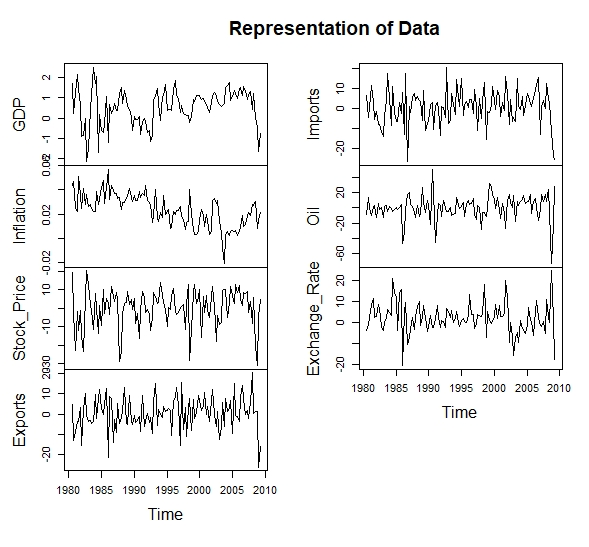
\includegraphics[width=\linewidth]{repdata.jpg}
\caption{Represention of Data}
\label{das}
\end{figure}

\hypertarget{empirical-analysis}{%
\section{Empirical Analysis}\label{empirical-analysis}}

In this section, I discuss the main results from the empirical analysis
I performed. First, I discuss the process I followed setting up the
priors and the model configuration. After, I assess the convergence of
the Markov chain. Furthermore, the impulse response functions are
analyzed as well as the forecasting results.

\hypertarget{configuration}{%
\subsection{Configuration}\label{configuration}}

The BVAR is specified with Minnesota priors. The hyperparameter
\(\lambda\) has a Gamma distribution with a mode of 0.2 and a standard
deviation of 0.4, as well as an upper and lower bound of 5 and 0.0001,
respectively. The use of a gamma distribution is widely used as a
conjugate prior in Bayesian analysis. Two dummy priors are also
included: the sum of coefficients (\emph{soc}) and the single unit root
(\emph{sur}) prior. Both dummy observations have a gamma distribution
with a mode and a standard deviation equal to one. I chose to treat
\(\lambda\), \emph{soc} and \emph{sur} as hierarchical priors. On the
other hand, the hypermeters that are not treated hierarchically are
treated as fixed and is equal to their mode (\(\alpha\) being an example
of a fixed prior). Table \ref{hyp} shows the estimated values of the
hyperparameters after optimization.

\begin{table}
\begin{center}
\begin{tabular}{ |c|c|c| } 
 \hline
 \(\lambda\) & \emph{soc} & \emph{sur}\\ 
 \hline
 0.12497 & 1.09338 & 0.17862 \\
 \hline
\end{tabular}
\caption{Hyperparamter Value after Estimation}
 \label{hyp}
\end{center}
\end{table}

\hypertarget{assessing-markov-chain-convergence}{%
\subsection{Assessing Markov Chain
Convergence}\label{assessing-markov-chain-convergence}}

The assessment of the convergence of the Markov Chain Monte Carlo (MCMC)
algorithm is an important part to analyse the stability of the BVAR. To
explore the posterior hyperparameter space, the Metropolis-Hastings
algorithm is used. I specified 200 000 saved draws, of which the first
50 000 will be burned. Figure \ref{mcmc} displays the trace and density
of the maximum likelihood (\textbackslash emph\{ml) and the hierarchical
hyperparameters (\(\lambda\).

A trace plot graphs the parameter value against the number of
iterations. The trace plot informs you of whether the burn-in period is
long enough. For the trace plot, one expects to see random scatter
around the mean value meaning that the model has converged to its
stationary distribution. If there is a trend in the sample space, then
it implies that the parameter has not converged. The trace plot in
figure \ref{mcmc} shows satisfactory results for \(\lambda\) and the
maximum likelihood (\emph{ml}), implying that the chains are well mixed
and that the chain most probably reached the correct distribution. The
density plots use the kernel density estimate to display the probability
function of the macroeconomic variables. As can be seen in figure
\ref{mcmc},

\begin{figure}[h]
\centering
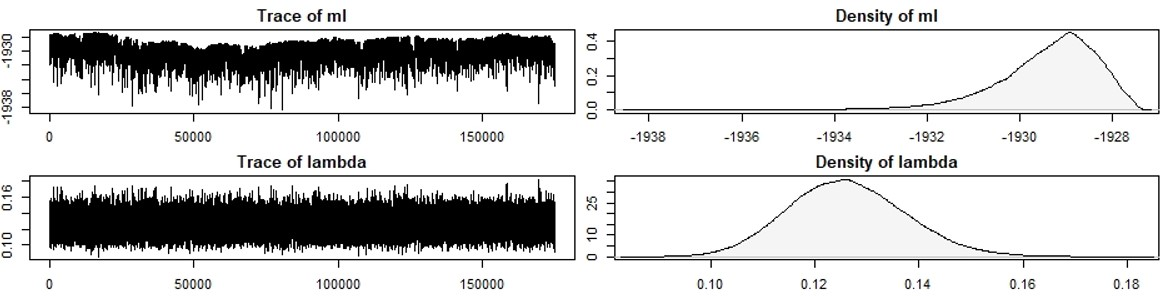
\includegraphics[width=\linewidth]{traced.jpg}
\caption{Trace and density plot of the maximum likelihood and the hierarchical hyperparameters }
\label{mcmc}
\end{figure}

\hypertarget{residual-plots}{%
\subsection{Residual Plots}\label{residual-plots}}

Figure \ref{resid} displays the residual plots for all the macroeconomic
variables. The residuals plots are used to ensure that the errors are
independently and normally distributed. The residuals values are
displayed on the y-axis and the fitted values on the x-axis. We would
expect to see that the residuals are centred on zero, indicating that
the model's predictions are correct on average.

\begin{figure}[h]
\centering
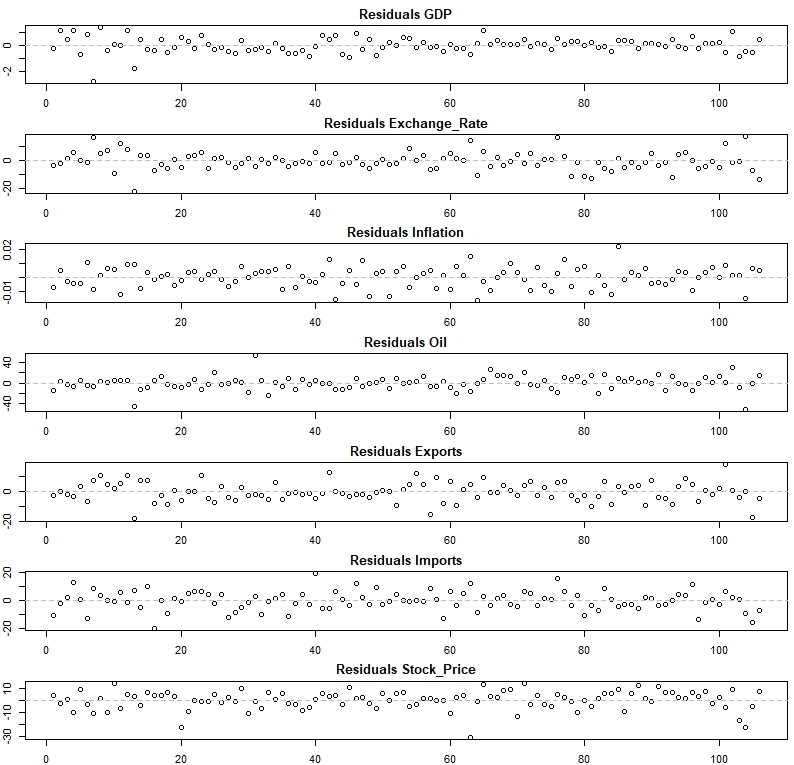
\includegraphics[width=\linewidth]{resid.jpg}
\caption{Residual Plots}
\label{resid}
\end{figure}

\newpage

\hypertarget{impulse-response-function}{%
\subsection{Impulse response function}\label{impulse-response-function}}

Impulse response functions describe the progress of a variable along a
specified time horizon after a specified shock has occurred. Figure
\ref{irf} displays how GDP, Inflation and Oil respond to a shock of all
seven macroeconomic variables described in section 4.

A positive shock to GDP, also interpreted as a supply shock, has a
positive effect on output causing prices to decrease. A supply shock
leads to an initial large increase in the supply of money, but also a
decrease in purchasing power. Therefore, inflation increases. A supply
shock can also be interpreted as a positive disruption of production
which will raise production costs and lead to an increase in oil prices.
As prices adjust, GDP and oil slowly return to their steady state, and
the initial impact on inflation is long-lasting.

A positive exchange rate shock has a positive and negative effects on
the South African economy. An increase in the exchange rates means that
exports are more expensive and decrease the price of imports. As a
result, there will be a decrease in demand for domestic products from
foreign markets leading to a decrease in GDP. However, the effect on GDP
from a positive exchange rate shock cancels out after 15 periods as GDP
returns to its steady-state. A positive exchange rate shock will have a
direct negative effect on inflation and a temporary negative effect on
the oil price.

An inflationary shock occurs when there is a sudden increase in the
prices of commodities. When nominal interest rates are held constant, a
positive inflationary shock will have a small negative effect on GDP.
This implies that an increase in nominal household wealth is less than
the increase in the price level, therefore real wealth falls. Oil price
and the level of inflation are often observed to move in the same
direction. An inflationary shock leads to a large, short-lived, increase
in the oil price, with the oil price returning to its steady-state after
eight periods.

Oil is an extremely important commodity that severely affects the global
market. An oil shock can be challenging to analyse since the reason
behind the shock is important. A positive oil price shock decreases
output and negatively affects spending and production patterns.
Therefore, South Africa will experience a temporary decrease in GDP.
Furthermore, an oil shock seems to have a small, relatively
insignificant effect on inflation. The impact on GDP and inflation
become smaller over time until both macroeconomic variables are back to
their steady states. However, South Africa does have the opportunity to
improve its net energy position which will lead to the country being
less vulnerable to oil
shocks\footnote{This was discussed at the recent COP26 conference}.

Increasing trade has been extremely important for South Africa. A trade
surplus contributes to economic growth. When the total amount of exports
exceeds the total amount total of imports it implies a high level of
output and an increase in productivity. An increase in imports is
positively related to GDP, while exports are negatively related to it.
This implies that the South African government should encourage trading
of goods and services internally, with exporting goods not being the
primary goal since it decreases GDP. A positive shock to imports and
exports seem to have an insignificant initial impact on the oil price.

A rising stock market usually means that the economy is growing and
leads to greater investor confidence. The increase in wealth experienced
by consumers leads to an increase in spending and purchasing power.
However, since the stock market is volatile, the effect of a positive
shock is usually short-lived, with GDP returning to its steady-state
after eleven periods. Since a positive shock to the stock market is
accompanied by an increase in spending, it can create an increase in
inflation if the demand for goods and services is considerably larger
than the supply. Furthermore, stock prices and oil prices tend to move
in the same direction, therefore a positive shock to the stock market
leads to a large, however short-lived, increase in the oil price.

\begin{figure}[h]
\centering
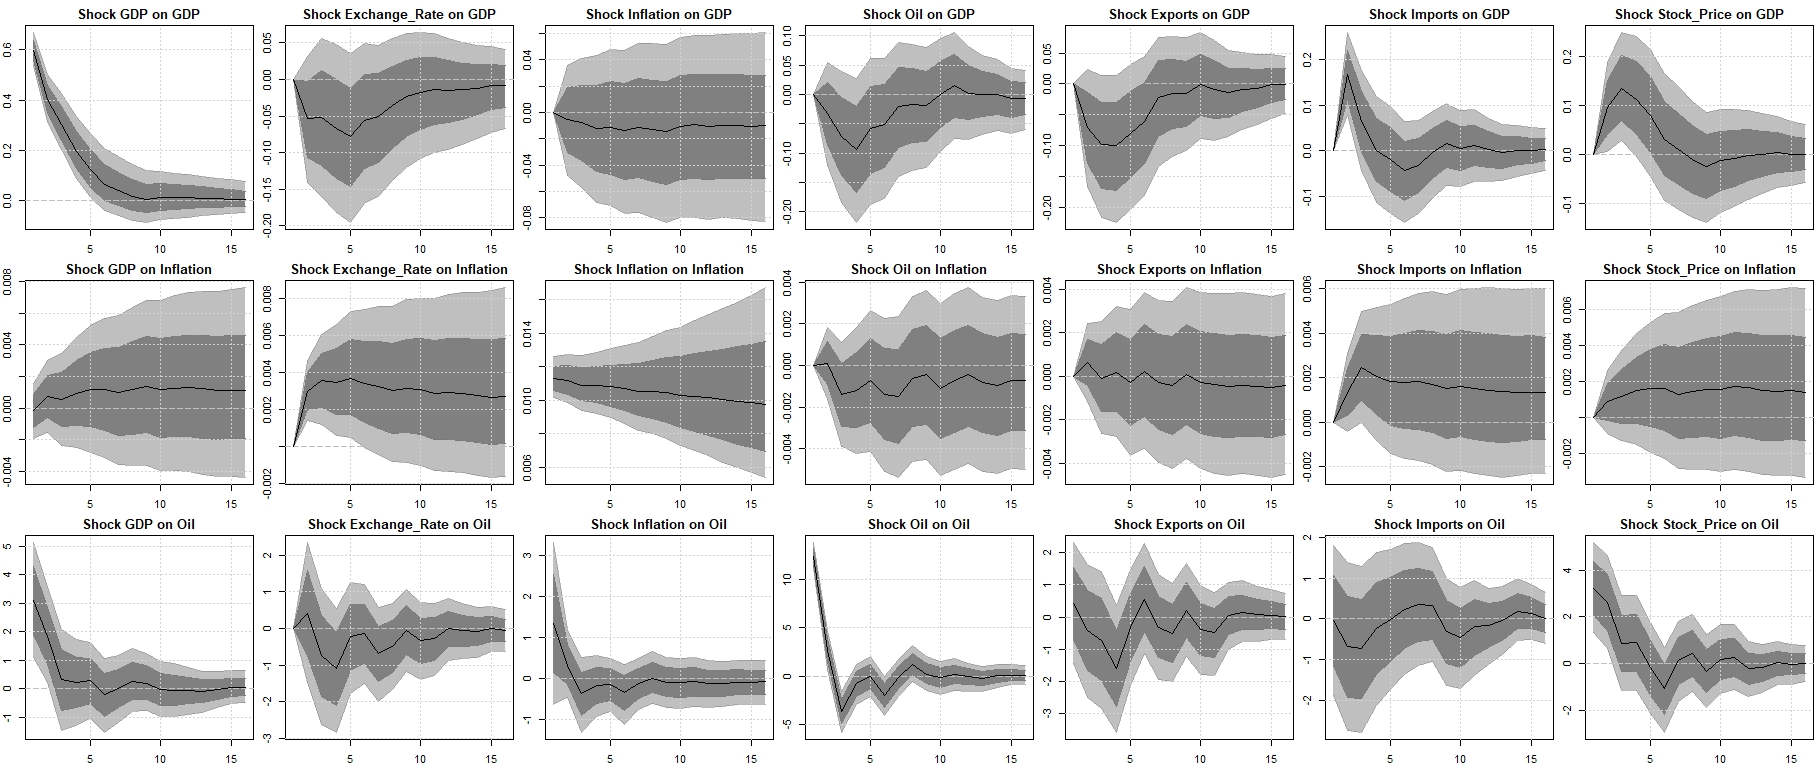
\includegraphics[scale = 0.45, angle = 90]{use_shocks.jpg}
\caption{Impulse Response Functions}
\label{irf}
\end{figure}

\hypertarget{forecasting}{%
\subsection{Forecasting}\label{forecasting}}

To forecast the model, I split the data into a training and a testing
set. Out of the 99 quarterly observations, the first 89 variables are
put into the training dataset and the last 10 variables are put into the
testing set. Therefore, the training set contains quarterly data from
1980:Q3 to 2004:Q4 and the testing set contains data from 2005:Q1 to
2007:Q2. To analyse the BVAR, I compare the forecasting results with a
VAR. The actual values of the data are displayed in table \ref{gdp10p}
in the appendix. Figure \ref{123} displays the forecast results for the
BVAR model for GDP, inflation and the oil price and figure \ref{1234}
displays the forecasting results for the VAR model.

\begin{figure}[h]
\centering
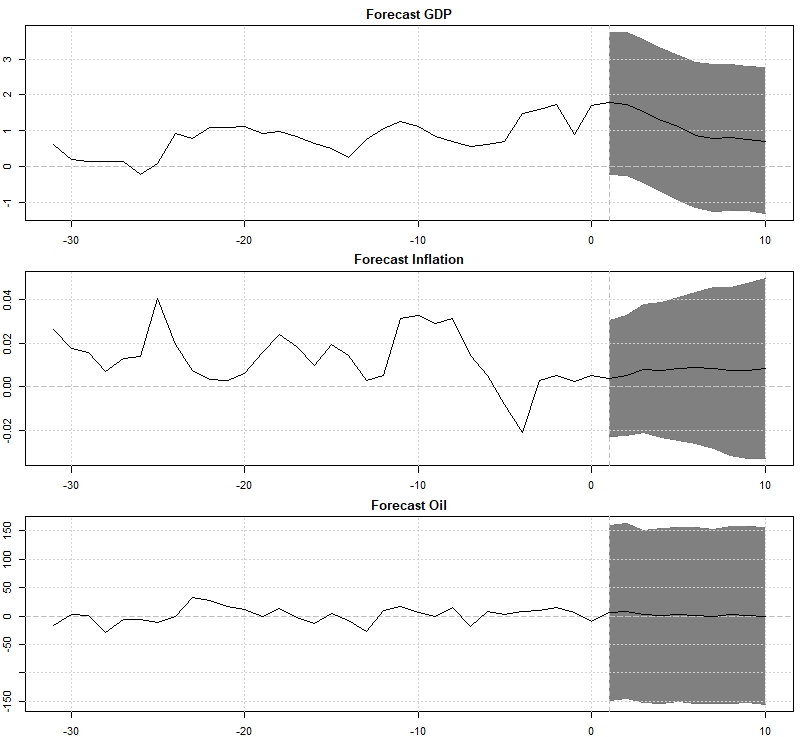
\includegraphics[scale = 0.6]{for1.jpg}
\caption{BVAR forecasting results}
\label{123}
\end{figure}

\begin{figure}[h]
\centering
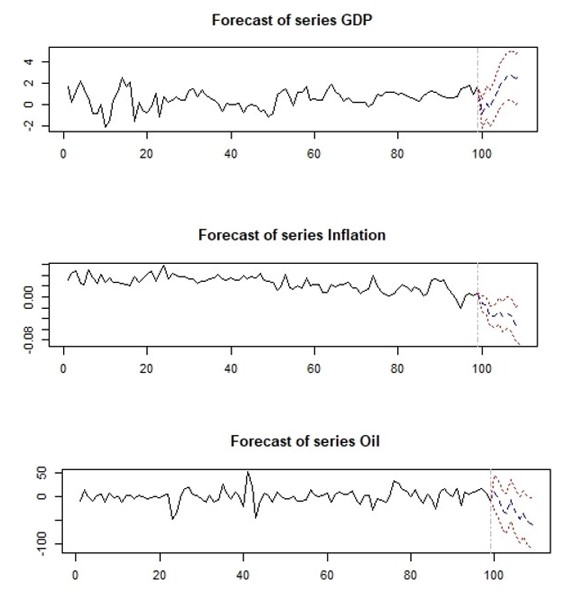
\includegraphics[scale = 0.8]{forcast.jpg}
\caption{VAR forecasting results}
\label{1234}
\end{figure}

Table \ref{gdpstat} displays statistic results to estimate and compare
the accuracy of the two models. The Mean Square Error (\emph{MSE}) is
the average square of the difference between the predicted values and
the actual values. The BVAR model produces smaller statistical results
than the VAR model, indicating that the BVAR produces more efficient
results. The Root Mean Square Error (\emph{RMSE}) calculates the
standard deviations of the residuals. It provides information about the
performance of the model by comparing the predicted value to the actual
value. The smaller the value, the better the model's performance. The
\emph{RMSE} statistic indicates that the BVAR model performs better than
the BAR model. The Mean Absolute Error (\emph{MAE}) computes the average
absolute difference between the predicted values and the observed
values. It measures the accuracy for continuous-time series variables.
For forecasting, you will want the \emph{MAE} to be as low as possible.
Therefore, the \emph{MAE} statistic shows that the BVAR model provides a
much more accurate forecast than the VAR model for all variables. It is
important to note that the \emph{MAE} statistic for the oil price is
extremely high for both models, suggesting that other models should be
explored if economic agents want to forecast the oil price.

There are two Theil-U statistics, the first measurement
(\emph{TheilU:1}) measures the forecast accuracy. The second measurement
(\emph{TheilU:2}) measures the forecast quality. The BVAR model has a
TheilU statistics of less than one for all three variables. This means
that the BVAR forecast is better than guessing. However, the TheilU
statistics for the VAR model is more than one, suggesting that the model
makes very poor predictions.

\begin{table}
\begin{center}
\begin{tabular}{|c|c|c|} 
  \hline
 Statistic & BVAR & VAR \\ 
 \hline
 \multicolumn{3}{|c|}{GDP} \\
 \hline
MSE & 0.1892822 & 1.745656 \\
RMSE & 0.4350658 & 1.321233 \\
MAE & 0.3997396 & 1.213998 \\
TheilU:1 & 0.1761636 & 0.423099 \\
TheilU:2 & 0.3439547 & 1.044541 \\
\hline
\multicolumn{3}{|c|}{Inflation} \\
 \hline
 MSE & 2.706111e-05 & 0.002002638 \\
RMSE & 0.005202029 & 0.04475084 \\
MAE & 0.003930009 & 0.04227154 \\
TheilU:1 & 0.2885939 & 0.9826374 \\
TheilU:2 & 0.4883881 & 4.201395 \\
\hline
\multicolumn{3}{|c|}{Oil Price} \\
 \hline
MSE & 87.49288 & 1591.65 \\
RMSE & 9.353763 & 39.89549 \\
MAE & 8.182195 & 34.72016 \\
TheilU:1 & 0.6246275 & 0.8361373 \\
TheilU:2 & 0.8281177 & 3.532072 \\
\hline
\end{tabular}
\caption{Forecasting Statistics }
 \label{gdpstat}
\end{center}
\end{table}

\hypertarget{diagnostics}{%
\section{Diagnostics}\label{diagnostics}}

In this section, I will preform numerous diagnostic and robustness test
to determine whether the validity and robustness of the BVAR that was
forecasted in section five. I test for stationary and the I analysize
the optimal number of lags.

\hypertarget{stationarity}{%
\subsection{Stationarity}\label{stationarity}}

Before preceding to analyse macroeconomic variables, it is important to
ensure that the variables are stationary. Having non-stationary time
series data can lead to spurious results implying that the stationarity
of macroeconomic time series data can significantly affect forecasting
behaviour \protect\hyperlink{ref-van}{Van Greunen, Heymans, Van Heerden
\& Van Vuuren} (\protect\hyperlink{ref-van}{2014}). I log and first
difference all variables, except inflation, to ensure stationarity. I
perform three robustness checks to confirm stationarity. First, I plot
the autocorrelation function (ACF) for each macroeconomic variable. The
ACF, displayed in figure \ref{autoc} describes the relationship between
the average data points and the preceding data points. On the x-axis,
you will have the number of lags and on the y-axis, you will have your
autocorrelation value. For all variables, except inflation, we notice
there is a significant spike at lag one and much lower subsequent lags.
Inflation also has a significant spike at lag one, followed by slightly
lower, and to some degree constant spikes. Except for inflation, all
variables degrade to zero rapidly, confirming stationarity. Figure
/ref\{autoc\} implies that inflation is non-stationary and should be
further investigated.

\begin{figure}[h]
\centering
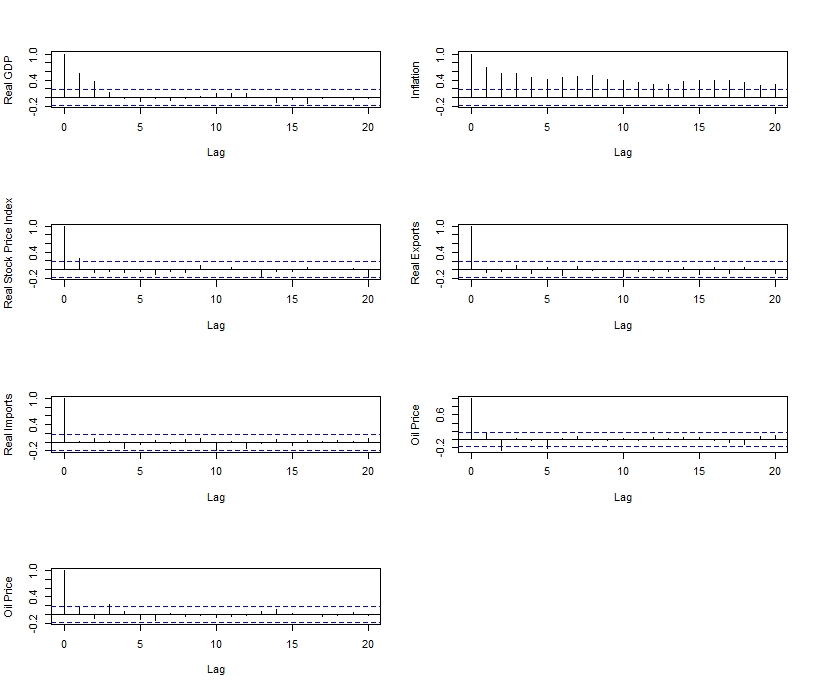
\includegraphics[width=\linewidth]{station.jpg}
\caption{Autocorrelation Function Analysis}
\label{autoc}
\end{figure}

To further investigate the stationarity of the macroeconomic variables,
I perform the Augmented Dickey-Fuller (ADF) test, with no trend since I
detrended the variables. The results are displayed in table \ref{adf}.
The null hypothesis states that a unit root is present in the time
series data and the alternative hypothesis states that the data is
stationary. The results show a p-value of less than 0.05 for all
variables, implying that we can reject the null hypothesis. Thereby, an
indication that the series is stationary

\begin{table}
\begin{center}
\begin{tabular}{ |c|c|c| } 
 \hline
 Variable & ADF statistic & P-Value \\ 
 \hline
 GDP & -5.0533 & 0.01 \\ 
 Inflation & -3.7828 & 0.02224 \\
 Stock Price & -4.9269 & 0.01 \\
 Exports & -3.9242 & 0.01538 \\
 Imports & -4.7132 & 0.01 \\
 Oil & -6.4081 & 0.01 \\
 Exchange Rate & -4.4494 & 0.01 \\
 \hline
\end{tabular}
\caption{Augmented Dickey-Fuller Test Analysis}
 \label{adf}
\end{center}
\end{table}

The ADF test results have a high probability of a type I error, meaning
that they can falsely reject the null hypothesis. Therefore, it needs to
be interpreted with caution. To ensure the validity of the results, I
preform the Phillips-Perron (PP) test.

The PP test also tests whether a variable has a unit root. The advantage
of analysing the PP test is that it is non-parametric, meaning that it
does not require selecting the level of serial correlation as the ADR
does. The null hypothesis is that the variables contain a unit root, and
the alternative hypothesis is that the variable was generated by a
stationary process. The results in table \ref{pptest} indicate that all
macroeconomic variables are stationary.

\begin{table}
\begin{center}
\begin{tabular}{ |c|c|c| } 
 \hline
 Variable & PP statistic & P-Value \\ 
 \hline
 GDP & -53.825 & 0.01 \\ 
 Inflation & -61.525 & 0.01 \\
 Stock Price & -82.78 & 0.01 \\
 Exports & -122.93 & 0.01 \\
 Imports & -114.63 & 0.01 \\
 Oil & -80.848 & 0.01 \\
 Exchange Rate & -98.411 & 0.01 \\
 \hline
\end{tabular}
\caption{Phillips-Perron unit Root Test Analysis}
 \label{pptest}
\end{center}
\end{table}

\hypertarget{optimal-lag-length}{%
\subsection{Optimal lag length}\label{optimal-lag-length}}

Determining the lag length for a Bayesian VAR is an extremely important
econometric exercise. I considered four unique criteria to determine the
optimal autoregressive lag length. Among the criteria that are
considered is the Akaike Information Criterion (AIC), the Schwarz
Criterion (SC) also known as the Bayesian Information Criterion (BIC),
the Hannan Quinn (HQ) and the Final Prediction Error (FPE).
\protect\hyperlink{ref-garnitz}{Garnitz, Lehmann \& Wohlrabe}
(\protect\hyperlink{ref-garnitz}{2019}) found that model selection by
the AIC or SC leads to very parsimonious models in the majority of cases
for forecasting GDP growth. \protect\hyperlink{ref-liew}{Liew}
(\protect\hyperlink{ref-liew}{2004}) found that the AIC and FPE produce
superior results over other criteria. However, this study will follow
the recommendation of \protect\hyperlink{ref-gupta}{Gupta, Olson \&
Wohar} (\protect\hyperlink{ref-gupta}{2017}) and
\protect\hyperlink{ref-clark}{Clark \& McCracken}
(\protect\hyperlink{ref-clark}{2008}) and use the AIC lag criteria to
choose the optimal lag length.

\begin{table}
\begin{center}
\begin{tabular}{ |c|c|c|c| } 
 \hline
 AIC(n) & HQ(n) & SC(n) & FPE(n) \\ 
 \hline
 10 & 1 & 1 & 1\\ 
 \hline
\end{tabular}
\caption{lag length analysis}
 \label{lag}
\end{center}
\end{table}

\hypertarget{conclusion}{%
\section{Conclusion}\label{conclusion}}

It is crucial for monetary and fiscal policy makers to be able to make
accurate predictions about economic growth. Bayesian statistics have
become a popular tool to forecast important macroeconomic variables. In
this paper, I estimate a seven variable BVAR model and compare the
forecasting results with a VAR model. The diagnostic results show that
all variables are stationary and that a model with 10 lags is most
appropriate. The BVAR model is estimated with Minnesota priors and two
dummy priors. The empirical results validate that BVAR has an efficient
level of forecast accuracy and quality, and it preferred over the VAR.
Therefore, I conclude that a BVAR model can be highly useful for policy
analysis.

\newpage

\hypertarget{references}{%
\section*{References}\label{references}}
\addcontentsline{toc}{section}{References}

\hypertarget{refs}{}
\begin{CSLReferences}{1}{0}
\leavevmode\vadjust pre{\hypertarget{ref-aron2002}{}}%
Aron, J. \& Muellbauer, J. 2002. Interest rate effects on output:
Evidence from a GDP forecasting model for south africa. \emph{IMF Staff
papers}. 49(1):185--213.

\leavevmode\vadjust pre{\hypertarget{ref-azmi}{}}%
Azmi, F. 2013. An empirical analysis of the relationship between GDP and
unemployment, interest rate and government spending. \emph{Interest Rate
and Government Spending (June 10, 2013)}.

\leavevmode\vadjust pre{\hypertarget{ref-can2011}{}}%
Canova, F. 2011. 10. Bayesian VARs. In Princeton University Press
\emph{Methods for applied macroeconomic research}. 373--417.

\leavevmode\vadjust pre{\hypertarget{ref-car2010}{}}%
Caraiani, P. et al. 2010. Forecasting romanian GDP using a BVAR model.
\emph{Romanian Journal of Economic Forecasting}. 13(4):76--87.

\leavevmode\vadjust pre{\hypertarget{ref-cepni}{}}%
Cepni, O., Güney, I.E. \& Swanson, N.R. 2019. Nowcasting and forecasting
GDP in emerging markets using global financial and macroeconomic
diffusion indexes. \emph{International Journal of Forecasting}.
35(2):555--572.

\leavevmode\vadjust pre{\hypertarget{ref-chama}{}}%
Chama-Chiliba, M.C., Gupta, R., Nkambule, N., Tlotlego, N., et al. 2012.
Forecasting key macroeconomic variables of the south african economy
using bayesian variable selection. \emph{Journal of Applied
Sciences(Faisalabad)}. 12(7):645--652.

\leavevmode\vadjust pre{\hypertarget{ref-clark}{}}%
Clark, T.E. \& McCracken, M.W. 2008. \emph{Forecasting with small
macroeconomic VARs in the presence of instabilities}. Emerald Group
Publishing Limited.

\leavevmode\vadjust pre{\hypertarget{ref-garnitz}{}}%
Garnitz, J., Lehmann, R. \& Wohlrabe, K. 2019. Forecasting GDP all over
the world using leading indicators based on comprehensive survey data.
\emph{Applied Economics}. 51(54):5802--5816.

\leavevmode\vadjust pre{\hypertarget{ref-2015prior}{}}%
Giannone, D., Lenza, M. \& Primiceri, G.E. 2015. Prior selection for
vector autoregressions. \emph{Review of Economics and Statistics}.
97(2):436--451.

\leavevmode\vadjust pre{\hypertarget{ref-greenwood}{}}%
Greenwood-Nimmo, M., Nguyen, V.H. \& Shin, Y. 2012. Probabilistic
forecasting of output growth, inflation and the balance of trade in a
GVAR framework. \emph{Journal of Applied Econometrics}. 27(4):554--573.

\leavevmode\vadjust pre{\hypertarget{ref-gupta}{}}%
Gupta, R., Olson, E. \& Wohar, M.E. 2017. Forecasting key US
macroeconomic variables with a factor-augmented qual VAR. \emph{Journal
of Forecasting}. 36(6):640--650.

\leavevmode\vadjust pre{\hypertarget{ref-kabundi}{}}%
Kabundi, A., Nel, E., Ruch, F., et al. 2016. Nowcasting real GDP growth
in south africa. \emph{Economic Research Southern Africa.{[}Working
Paper, No. 581.{]} Pretoria: National Treasury of South Africa}.

\leavevmode\vadjust pre{\hypertarget{ref-liew}{}}%
Liew, V.K.-S. 2004. Which lag length selection criteria should we
employ? \emph{Economics bulletin}. 3(33):1--9.

\leavevmode\vadjust pre{\hypertarget{ref-litter}{}}%
Litterman, R.B. 1980. \emph{Bayesian procedure for forecasting with
vector autoregressions}. Massachusetts Institute of Technology.

\leavevmode\vadjust pre{\hypertarget{ref-mamo}{}}%
Mamo, F. 2012.

\leavevmode\vadjust pre{\hypertarget{ref-nkomo}{}}%
Nkomo, J.C. 2006. The impact of higher oil prices on southern african
countries. \emph{Journal of Energy in Southern Africa}. 17(1):10--17.

\leavevmode\vadjust pre{\hypertarget{ref-sacak}{}}%
Sacakli-Sacildi, I. 2015. Do BVAR models forecast turkish GDP better
than UVAR models? \emph{Journal of Economics, Management and Trade}.
259--268.

\leavevmode\vadjust pre{\hypertarget{ref-sims1980}{}}%
Sims, C.A. 1980. Macroeconomics and reality. \emph{Econometrica: journal
of the Econometric Society}. 1--48.

\leavevmode\vadjust pre{\hypertarget{ref-stock2001}{}}%
Stock, J.H. \& Watson, M.W. 2001. Vector autoregressions. \emph{Journal
of Economic perspectives}. 15(4):101--115.

\leavevmode\vadjust pre{\hypertarget{ref-trem}{}}%
Tremblay, R. 1990. The "export-import" effect and economic growth.
\emph{North American Review of Economics and Finance}. 1(2):241--252.

\leavevmode\vadjust pre{\hypertarget{ref-van}{}}%
Van Greunen, J., Heymans, A., Van Heerden, C. \& Van Vuuren, G. 2014.
The prominence of stationarity in time series forecasting. \emph{Studies
in Economics and Econometrics}. 38(1):1--16.

\end{CSLReferences}

\hypertarget{appendix}{%
\section*{Appendix}\label{appendix}}
\addcontentsline{toc}{section}{Appendix}

\begin{table}
\begin{center}
\begin{tabular}{|c|c|c|c|} 
 \hline
 Date & Actual & Forecast BVAR & Forecast VAR\\ 
 \hline
  \multicolumn{4}{|c|}{GDP} \\
 \hline
2005Q1 & 1.3641975 & 1.7448787 & - 0.8908903 \\
2005Q2 & 1.2130095 & 1.7434149 & 0.1065763 \\
2005Q3 & 0.9688178 & 1.5251118 & -0.3492994 \\
2005Q4 & 1.4387614 & 1.2852046 & 0.4464542 \\
2006Q1 & 1.4957687 & 1.1148588 & 1.5528151 \\
2006Q2 & 1.1248029 & 0.8768851 & 2.1273837 \\
2006Q3 & 1.5373958 & 0.8314630 & 2.6274903 \\
2006Q4 & 1.3361993 & 0.8156417 & 2.6859277 \\
2007Q1 & 0.8991781 & 0.7431564 & 2.3765362 \\
2007Q2 & 1.0947265 & 0.7296073 & 2.5859514 \\
 \hline
\multicolumn{4}{|c|}{Inflation} \\
\hline
2005Q1 & 0.006368598 & 0.004051628 & -0.01265742 \\
2005Q2 & 0.005283041 & 0.005142886 & -0.01726220 \\
2005Q3 & 0.006773210 & 0.008334394 & -0.03529701 \\
2005Q4 & 0.002397284 & 0.007580780 & -0.03532820 \\
2006Q1 & 0.005726190 & 0.007872427 & -0.02663917 \\
2006Q2 & 0.009536616 & 0.008883043 & -0.03608311 \\
2006Q3 & 0.018747035 & 0.007656673 & -0.02982121\\
2006Q4 & 0.010118324 & 0.006849587 & -0.03457038 \\
2007Q1 & 0.011258538 & 0.007385887 & -0.05109997 \\
2007Q2 & 0.017610026 & 0.008543302 & -0.05013784 \\
\hline
\multicolumn{4}{|c|}{Oil Price} \\
\hline
2005Q1 & 8.0106647 & 3.83536202 & 9.715215 \\
2005Q2 & 17.6070462 & 8.95983541 & -5.681085\\
2005Q3 & -7.7909729 & -0.01693524 & -31.130308 \\
2005Q4 & 8.3794895 & 0.41643603 & -34.810443 \\
2006Q1 & 12.0328698 & 5.41052479 & -8.030314 \\
2006Q2 & 0.3763495 & 0.85631826 & -33.676059 \\
2006Q3 & -16.0104983 & 0.23662992 & -48.439894 \\
2006Q4 & -2.8129879 & 2.94611692 & -35.927783 \\
2007Q1 & 16.8641448 & 1.18515221 & -51.381779 \\
2007Q2 & 8.7831482 & 0.30833741 & -58.990796 \\
\hline 
\end{tabular}
\caption{10 period ahead forecast results }
 \label{gdp10p}
\end{center}
\end{table}

\bibliography{Tex/ref}





\end{document}
